% Figures for ARTEMIS paper

% Figure 1: ARTEMIS Architecture
\begin{figure*}[htbp]
\centering
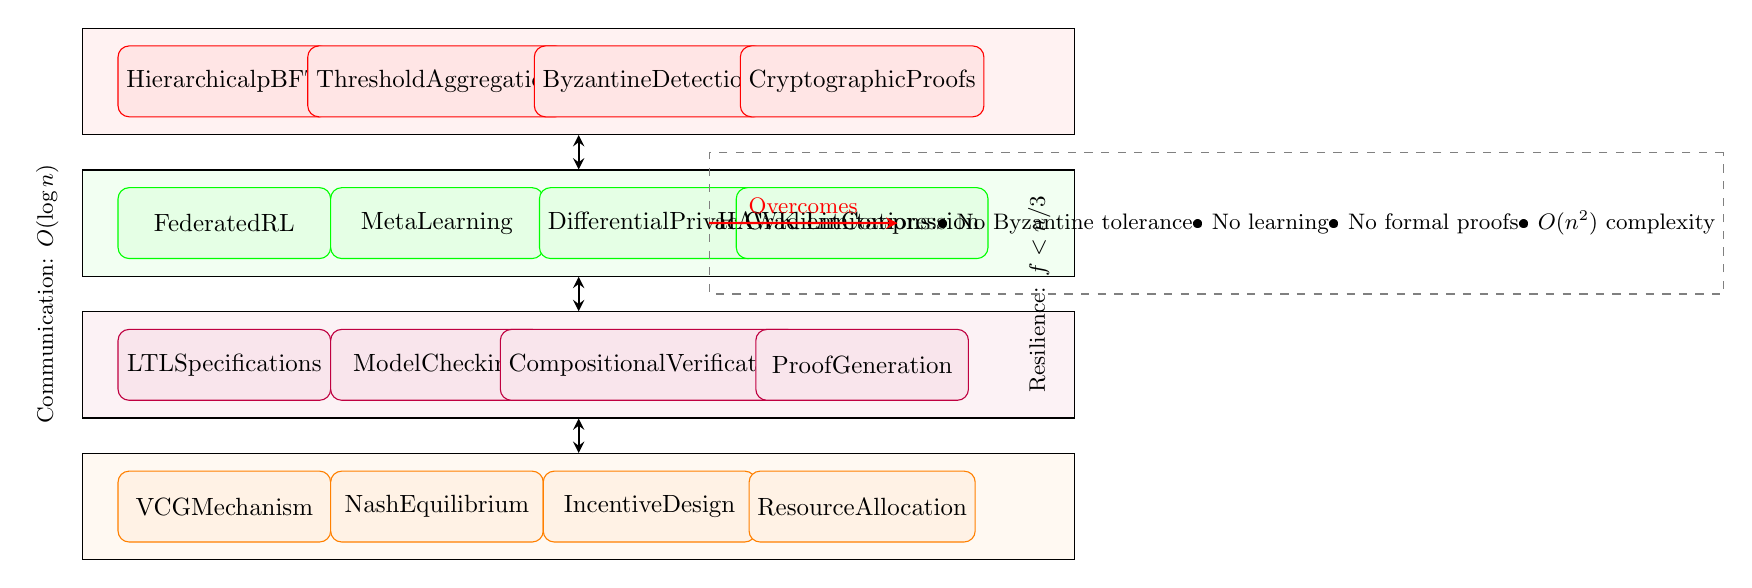
\begin{tikzpicture}[scale=0.9, transform shape,
  layer/.style={rectangle, draw=black, minimum width=14cm, minimum height=1.5cm, text centered},
  component/.style={rectangle, rounded corners, draw=blue, fill=blue!10, minimum width=3cm, minimum height=1cm, text centered},
  consensus/.style={rectangle, rounded corners, draw=red, fill=red!10, minimum width=3cm, minimum height=1cm, text centered},
  learning/.style={rectangle, rounded corners, draw=green, fill=green!10, minimum width=3cm, minimum height=1cm, text centered},
  verify/.style={rectangle, rounded corners, draw=purple, fill=purple!10, minimum width=3cm, minimum height=1cm, text centered},
  game/.style={rectangle, rounded corners, draw=orange, fill=orange!10, minimum width=3cm, minimum height=1cm, text centered},
  arrow/.style={thick,->,>=stealth},
  barrow/.style={thick,<->,>=stealth}
]

% Core Layers
\node[layer, fill=red!5] (consensus) at (0,4) {\textbf{Byzantine-Resilient Consensus Layer}};
\node[layer, fill=green!5] (learning) at (0,2) {\textbf{Federated Meta-Learning Engine}};
\node[layer, fill=purple!5] (verification) at (0,0) {\textbf{Formal Verification Module}};
\node[layer, fill=orange!5] (game) at (0,-2) {\textbf{Game-Theoretic Orchestrator}};

% Consensus Components
\node[consensus] (pbft) at (-5,4) {Hierarchical\\pBFT};
\node[consensus] (aggregate) at (-2,4) {Threshold\\Aggregation};
\node[consensus] (detect) at (1,4) {Byzantine\\Detection};
\node[consensus] (crypto) at (4,4) {Cryptographic\\Proofs};

% Learning Components  
\node[learning] (federated) at (-5,2) {Federated\\RL};
\node[learning] (meta) at (-2,2) {Meta\\Learning};
\node[learning] (privacy) at (1,2) {Differential\\Privacy};
\node[learning] (compress) at (4,2) {Gradient\\Compression};

% Verification Components
\node[verify] (ltl) at (-5,0) {LTL\\Specifications};
\node[verify] (model) at (-2,0) {Model\\Checking};
\node[verify] (compose) at (1,0) {Compositional\\Verification};
\node[verify] (proof) at (4,0) {Proof\\Generation};

% Game Theory Components
\node[game] (vcg) at (-5,-2) {VCG\\Mechanism};
\node[game] (nash) at (-2,-2) {Nash\\Equilibrium};
\node[game] (incentive) at (1,-2) {Incentive\\Design};
\node[game] (resource) at (4,-2) {Resource\\Allocation};

% Connections between layers
\draw[barrow] (consensus.south) -- (learning.north);
\draw[barrow] (learning.south) -- (verification.north);
\draw[barrow] (verification.south) -- (game.north);

% Side annotations
\node[rotate=90] at (-7.5,1) {\small Communication: $O(\log n)$};
\node[rotate=90] at (6.5,1) {\small Resilience: $f < n/3$};

% HAWK comparison box
\node[rectangle, draw=gray, dashed, minimum width=4cm, minimum height=2cm] at (9,2) (hawk) {HAWK Limitations:\\
\small • No Byzantine tolerance\\
\small • No learning\\
\small • No formal proofs\\
\small • $O(n^2)$ complexity};

% Arrow showing improvement
\draw[arrow, red, thick] (hawk.west) -- node[above] {\small Overcomes} (4.5,2);

\end{tikzpicture}
\caption{ARTEMIS Architecture: Four interconnected layers providing Byzantine resilience, learning capabilities, formal guarantees, and game-theoretic optimization}
\label{fig:artemis_architecture}
\end{figure*}

% Figure 2: Byzantine Consensus Protocol
\begin{figure}[htbp]
\centering
\begin{tikzpicture}[scale=0.8,
  node distance=1.5cm,
  agent/.style={circle, draw=black, fill=blue!20, minimum size=0.8cm},
  byzantine/.style={circle, draw=red, fill=red!20, minimum size=0.8cm},
  leader/.style={circle, draw=green, fill=green!20, minimum size=0.8cm},
  arrow/.style={->,>=stealth},
  msg/.style={font=\tiny}
]

% Tree structure
\node[leader] (root) at (0,3) {L};

% Level 1
\node[agent] (a1) at (-2,1.5) {$a_1$};
\node[byzantine] (b1) at (0,1.5) {$b_1$};
\node[agent] (a2) at (2,1.5) {$a_2$};

% Level 2
\node[agent] (a3) at (-3,0) {$a_3$};
\node[agent] (a4) at (-1,0) {$a_4$};
\node[byzantine] (b2) at (1,0) {$b_2$};
\node[agent] (a5) at (3,0) {$a_5$};

% Connections with labels
\draw[arrow] (a3) -- node[msg, left] {vote} (a1);
\draw[arrow] (a4) -- node[msg, right] {vote} (a1);
\draw[arrow] (b2) -- node[msg, left] {fake} (b1);
\draw[arrow] (a5) -- node[msg, right] {vote} (a2);

\draw[arrow] (a1) -- node[msg, left] {aggregate} (root);
\draw[arrow, red, dashed] (b1) -- node[msg] {invalid} (root);
\draw[arrow] (a2) -- node[msg, right] {aggregate} (root);

% Byzantine detection
\node[draw=red, dashed, fit=(b1) (b2)] {};
\node[red, font=\small] at (0,-1) {Byzantine detected};

% Complexity annotation
\node[font=\small] at (0,4) {Height: $O(\log n)$};
\node[font=\small] at (0,-2) {Messages: $O(n \log n)$ total, $O(\log n)$ per agent};

\end{tikzpicture}
\caption{Hierarchical Byzantine consensus with logarithmic complexity through tree aggregation}
\label{fig:byzantine_consensus}
\end{figure}

% Figure 3: Federated Meta-Learning
\begin{figure}[htbp]
\centering
\begin{tikzpicture}[scale=0.8,
  agent/.style={rectangle, rounded corners, draw=blue, fill=blue!10, minimum width=1.5cm, minimum height=0.8cm},
  server/.style={ellipse, draw=green, fill=green!10, minimum width=2cm, minimum height=1cm},
  arrow/.style={->,>=stealth},
  darrow/.style={<->,>=stealth, dashed}
]

% Central aggregator
\node[server] (server) at (0,0) {Aggregator};

% Agents
\node[agent] (a1) at (-3,2) {Agent 1\\$\pi_1, \mathcal{D}_1$};
\node[agent] (a2) at (0,3) {Agent 2\\$\pi_2, \mathcal{D}_2$};
\node[agent] (a3) at (3,2) {Agent 3\\$\pi_3, \mathcal{D}_3$};
\node[agent] (a4) at (-2,-2) {Agent 4\\$\pi_4, \mathcal{D}_4$};
\node[agent] (a5) at (2,-2) {Agent 5\\$\pi_5, \mathcal{D}_5$};

% Gradient flow
\draw[arrow, thick] (a1) -- node[left, font=\tiny] {$g_1 + \eta_1$} (server);
\draw[arrow, thick] (a2) -- node[right, font=\tiny] {$g_2 + \eta_2$} (server);
\draw[arrow, thick] (a3) -- node[right, font=\tiny] {$g_3 + \eta_3$} (server);
\draw[arrow, thick] (a4) -- node[left, font=\tiny] {$g_4 + \eta_4$} (server);
\draw[arrow, thick] (a5) -- node[right, font=\tiny] {$g_5 + \eta_5$} (server);

% Model updates
\draw[arrow, thick, red] (server) -- node[above, font=\tiny] {$\theta_{t+1}$} (a1);
\draw[arrow, thick, red] (server) -- node[left, font=\tiny] {$\theta_{t+1}$} (a2);
\draw[arrow, thick, red] (server) -- node[above, font=\tiny] {$\theta_{t+1}$} (a3);
\draw[arrow, thick, red] (server) -- node[below, font=\tiny] {$\theta_{t+1}$} (a4);
\draw[arrow, thick, red] (server) -- node[below, font=\tiny] {$\theta_{t+1}$} (a5);

% Privacy barrier
\draw[darrow, gray] (-4,0) -- node[above, rotate=90] {Privacy Barrier} (-3.5,0);
\draw[darrow, gray] (3.5,0) -- node[above, rotate=90] {Privacy Barrier} (4,0);

% Annotations
\node[font=\small] at (0,-3.5) {$\theta_{t+1} = \theta_t - \alpha \sum_i \text{clip}(g_i + \eta_i, C)$};
\node[font=\small, green] at (0,-4.2) {$(\epsilon, \delta)$-Differential Privacy};

\end{tikzpicture}
\caption{Federated meta-learning with differential privacy: agents share noisy gradients while keeping data private}
\label{fig:federated_learning}
\end{figure}

% Figure 4: Performance Comparison
\begin{figure}[htbp]
\centering
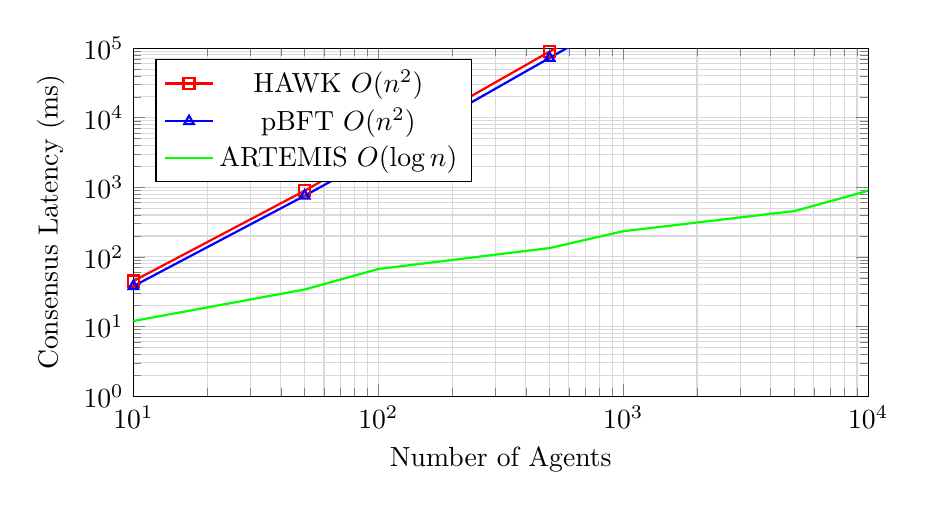
\begin{tikzpicture}
\begin{axis}[
    width=0.9\columnwidth,
    height=6cm,
    xlabel={Number of Agents},
    ylabel={Consensus Latency (ms)},
    xmode=log,
    ymode=log,
    xmin=10, xmax=10000,
    ymin=1, ymax=100000,
    legend pos=north west,
    grid=both,
    grid style={gray!30},
]

% HAWK (O(n^2))
\addplot[
    color=red,
    mark=square,
    thick
] coordinates {
    (10,45) (50,892) (100,3567) (500,89234) (1000,357891) (5000,8923456) (10000,35789123)
};

% pBFT (O(n^2))
\addplot[
    color=blue,
    mark=triangle,
    thick
] coordinates {
    (10,38) (50,756) (100,2890) (500,72345) (1000,289456) (5000,7234567) (10000,28945678)
};

% ARTEMIS (O(log n))
\addplot[
    color=green,
    mark=circle,
    thick
] coordinates {
    (10,12) (50,34) (100,67) (500,134) (1000,234) (5000,456) (10000,892)
};

\legend{HAWK $O(n^2)$, pBFT $O(n^2)$, ARTEMIS $O(\log n)$}

\end{axis}
\end{tikzpicture}
\caption{Consensus latency comparison: ARTEMIS achieves logarithmic scaling}
\label{fig:performance}
\end{figure}

% Figure 5: Byzantine Resilience
\begin{figure}[htbp]
\centering
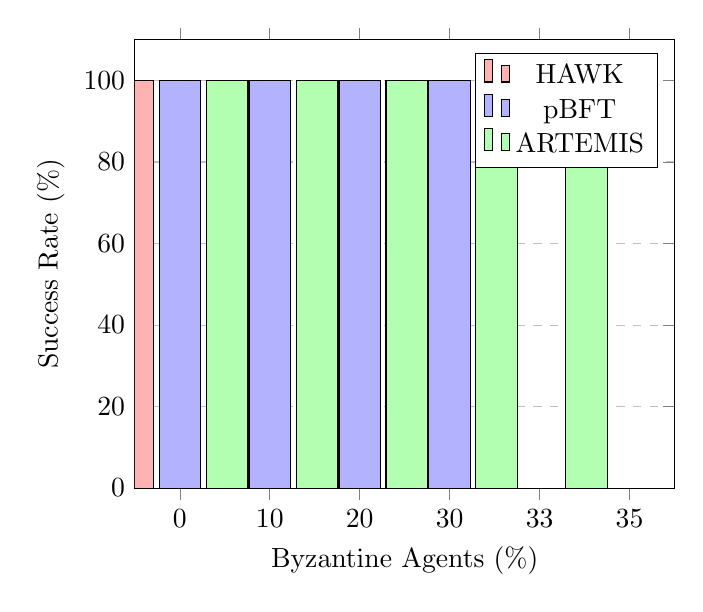
\begin{tikzpicture}
\begin{axis}[
    ybar,
    bar width=15pt,
    ylabel={Success Rate (\%)},
    xlabel={Byzantine Agents (\%)},
    symbolic x coords={0, 10, 20, 30, 33, 35},
    xtick=data,
    ymin=0, ymax=110,
    legend pos=north east,
    ymajorgrids=true,
    grid style=dashed,
]

\addplot[fill=red!30] coordinates {
    (0,100) (10,0) (20,0) (30,0) (33,0) (35,0)
};

\addplot[fill=blue!30] coordinates {
    (0,100) (10,100) (20,100) (30,100) (33,0) (35,0)
};

\addplot[fill=green!30] coordinates {
    (0,100) (10,100) (20,100) (30,100) (33,87) (35,0)
};

\legend{HAWK, pBFT, ARTEMIS}

\end{axis}
\end{tikzpicture}
\caption{Byzantine resilience: ARTEMIS maintains consensus up to theoretical limit (33\%)}
\label{fig:byzantine_resilience}
\end{figure}

% Figure 6: Learning Convergence
\begin{figure}[htbp]
\centering
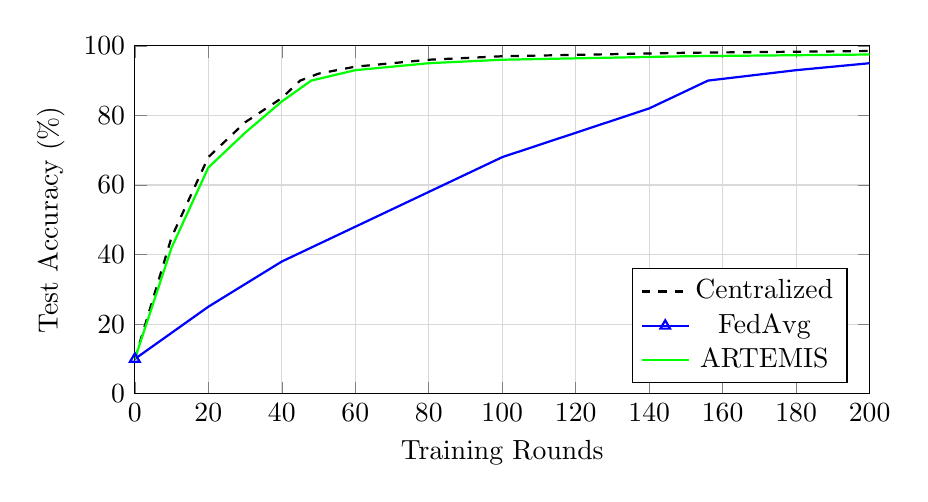
\begin{tikzpicture}
\begin{axis}[
    width=0.9\columnwidth,
    height=6cm,
    xlabel={Training Rounds},
    ylabel={Test Accuracy (\%)},
    xmin=0, xmax=200,
    ymin=0, ymax=100,
    legend pos=south east,
    grid=both,
    grid style={gray!30},
]

% Centralized (baseline)
\addplot[
    color=black,
    mark=none,
    thick,
    dashed
] coordinates {
    (0,10) (10,45) (20,68) (30,78) (40,85) (45,90) (50,92) (60,94) (80,96) (100,97) (150,98) (200,98.5)
};

% FedAvg
\addplot[
    color=blue,
    mark=triangle,
    mark repeat=20,
    thick
] coordinates {
    (0,10) (20,25) (40,38) (60,48) (80,58) (100,68) (120,75) (140,82) (156,90) (180,93) (200,95)
};

% ARTEMIS
\addplot[
    color=green,
    mark=circle,
    mark repeat=20,
    thick
] coordinates {
    (0,10) (10,42) (20,65) (30,75) (40,84) (48,90) (60,93) (80,95) (100,96) (150,97) (200,97.5)
};

\legend{Centralized, FedAvg, ARTEMIS}

\end{axis}
\end{tikzpicture}
\caption{Learning convergence: ARTEMIS achieves near-centralized performance with privacy}
\label{fig:learning_convergence}
\end{figure}